% ------------------------------------------------------------------------------
% TYPO3 CMS 8 LTS - What's New - Chapter "Form Framework" (English Version)
%
% @author	Michael Schams <schams.net>
% @license	Creative Commons BY-NC-SA 3.0
% @link		http://typo3.org/download/release-notes/whats-new/
% @language	English
% ------------------------------------------------------------------------------
% LTXE-CHAPTER-UID:		7b857ef8-be0a68dc-f93780d5-c5ae512e
% LTXE-CHAPTER-NAME:	Form Framework
% ------------------------------------------------------------------------------

\section{Form Framework}
\begin{frame}[fragile]
	\frametitle{Form Framework}

	\begin{center}\huge{\color{typo3darkgrey}\textbf{Form Framework}}\end{center}
	\begin{center}\large{\textit{Creating complex forms becomes a piece of cake}}\end{center}

\end{frame}

% ------------------------------------------------------------------------------
% LTXE-SLIDE-START
% LTXE-SLIDE-UID:		e00709d6-ccb8a4d0-1cca1d28-431a00a5
% LTXE-SLIDE-TITLE:		#77910: New Form Framework (1)
% ------------------------------------------------------------------------------
\begin{frame}[fragile]
	\frametitle{Form Framework}
	\framesubtitle{Main Facts}

	\begin{itemize}
		\item Flexible new framework for building forms was integrated
		\item Uses jQuery and a modern architecture, ensuring high flexibility and extensibility
		\item Replaces the legacy \textit{Form Wizard} based on ExtJS
		\item Forms are stored as templates, which can be re-used across the website
		\item Configuration stored in YAML files\newline
			\small(can be exported, adjusted, version controlled, shared, etc.)\normalsize
		\item Very intuitive to use (\textit{editors will love it!})
%		\item Demonstration video of a preview is available at YouTube:\newline
%			\url{https://www.youtube.com/watch?v=F9sTAOEcTI0}
	\end{itemize}

\end{frame}

% ------------------------------------------------------------------------------
% LTXE-SLIDE-START
% LTXE-SLIDE-UID:		72e78e2d-eda9d443-d07aa275-a60a53c6
% LTXE-SLIDE-TITLE:		#77910: New Form Framework (2)
% ------------------------------------------------------------------------------
\begin{frame}[fragile]
	\frametitle{Form Framework}
	\framesubtitle{Validators and Finishers}

	\begin{itemize}

		\item \textbf{Validators:}

			\begin{itemize}
				\item Data entered can be verified by \textit{Validators}
				\item Typical Validators are included in TYPO3 CMS
					(e.g. for fields such as email, alphanumeric, integer, regular expressions, etc.)
				\item Custom developed Validators can extend this functionality
			\end{itemize}

		\item \textbf{Finishers:}

			\begin{itemize}
				\item Control what should happen with the form data submitted
					(e.g. trigger an email, redirect to a page, etc.)
				\item Custom developed Finishers can extend this functionality
			\end{itemize}

	\end{itemize}

\end{frame}

% ------------------------------------------------------------------------------
% LTXE-SLIDE-START
% LTXE-SLIDE-UID:		3bbca669-629eab1c-0230fd06-71e7071c
% LTXE-SLIDE-TITLE:		#77910: New Form Framework (3)
% ------------------------------------------------------------------------------
\begin{frame}[fragile]
	\frametitle{Form Framework}
	\framesubtitle{Screenshot (1)}

	\begin{figure}
		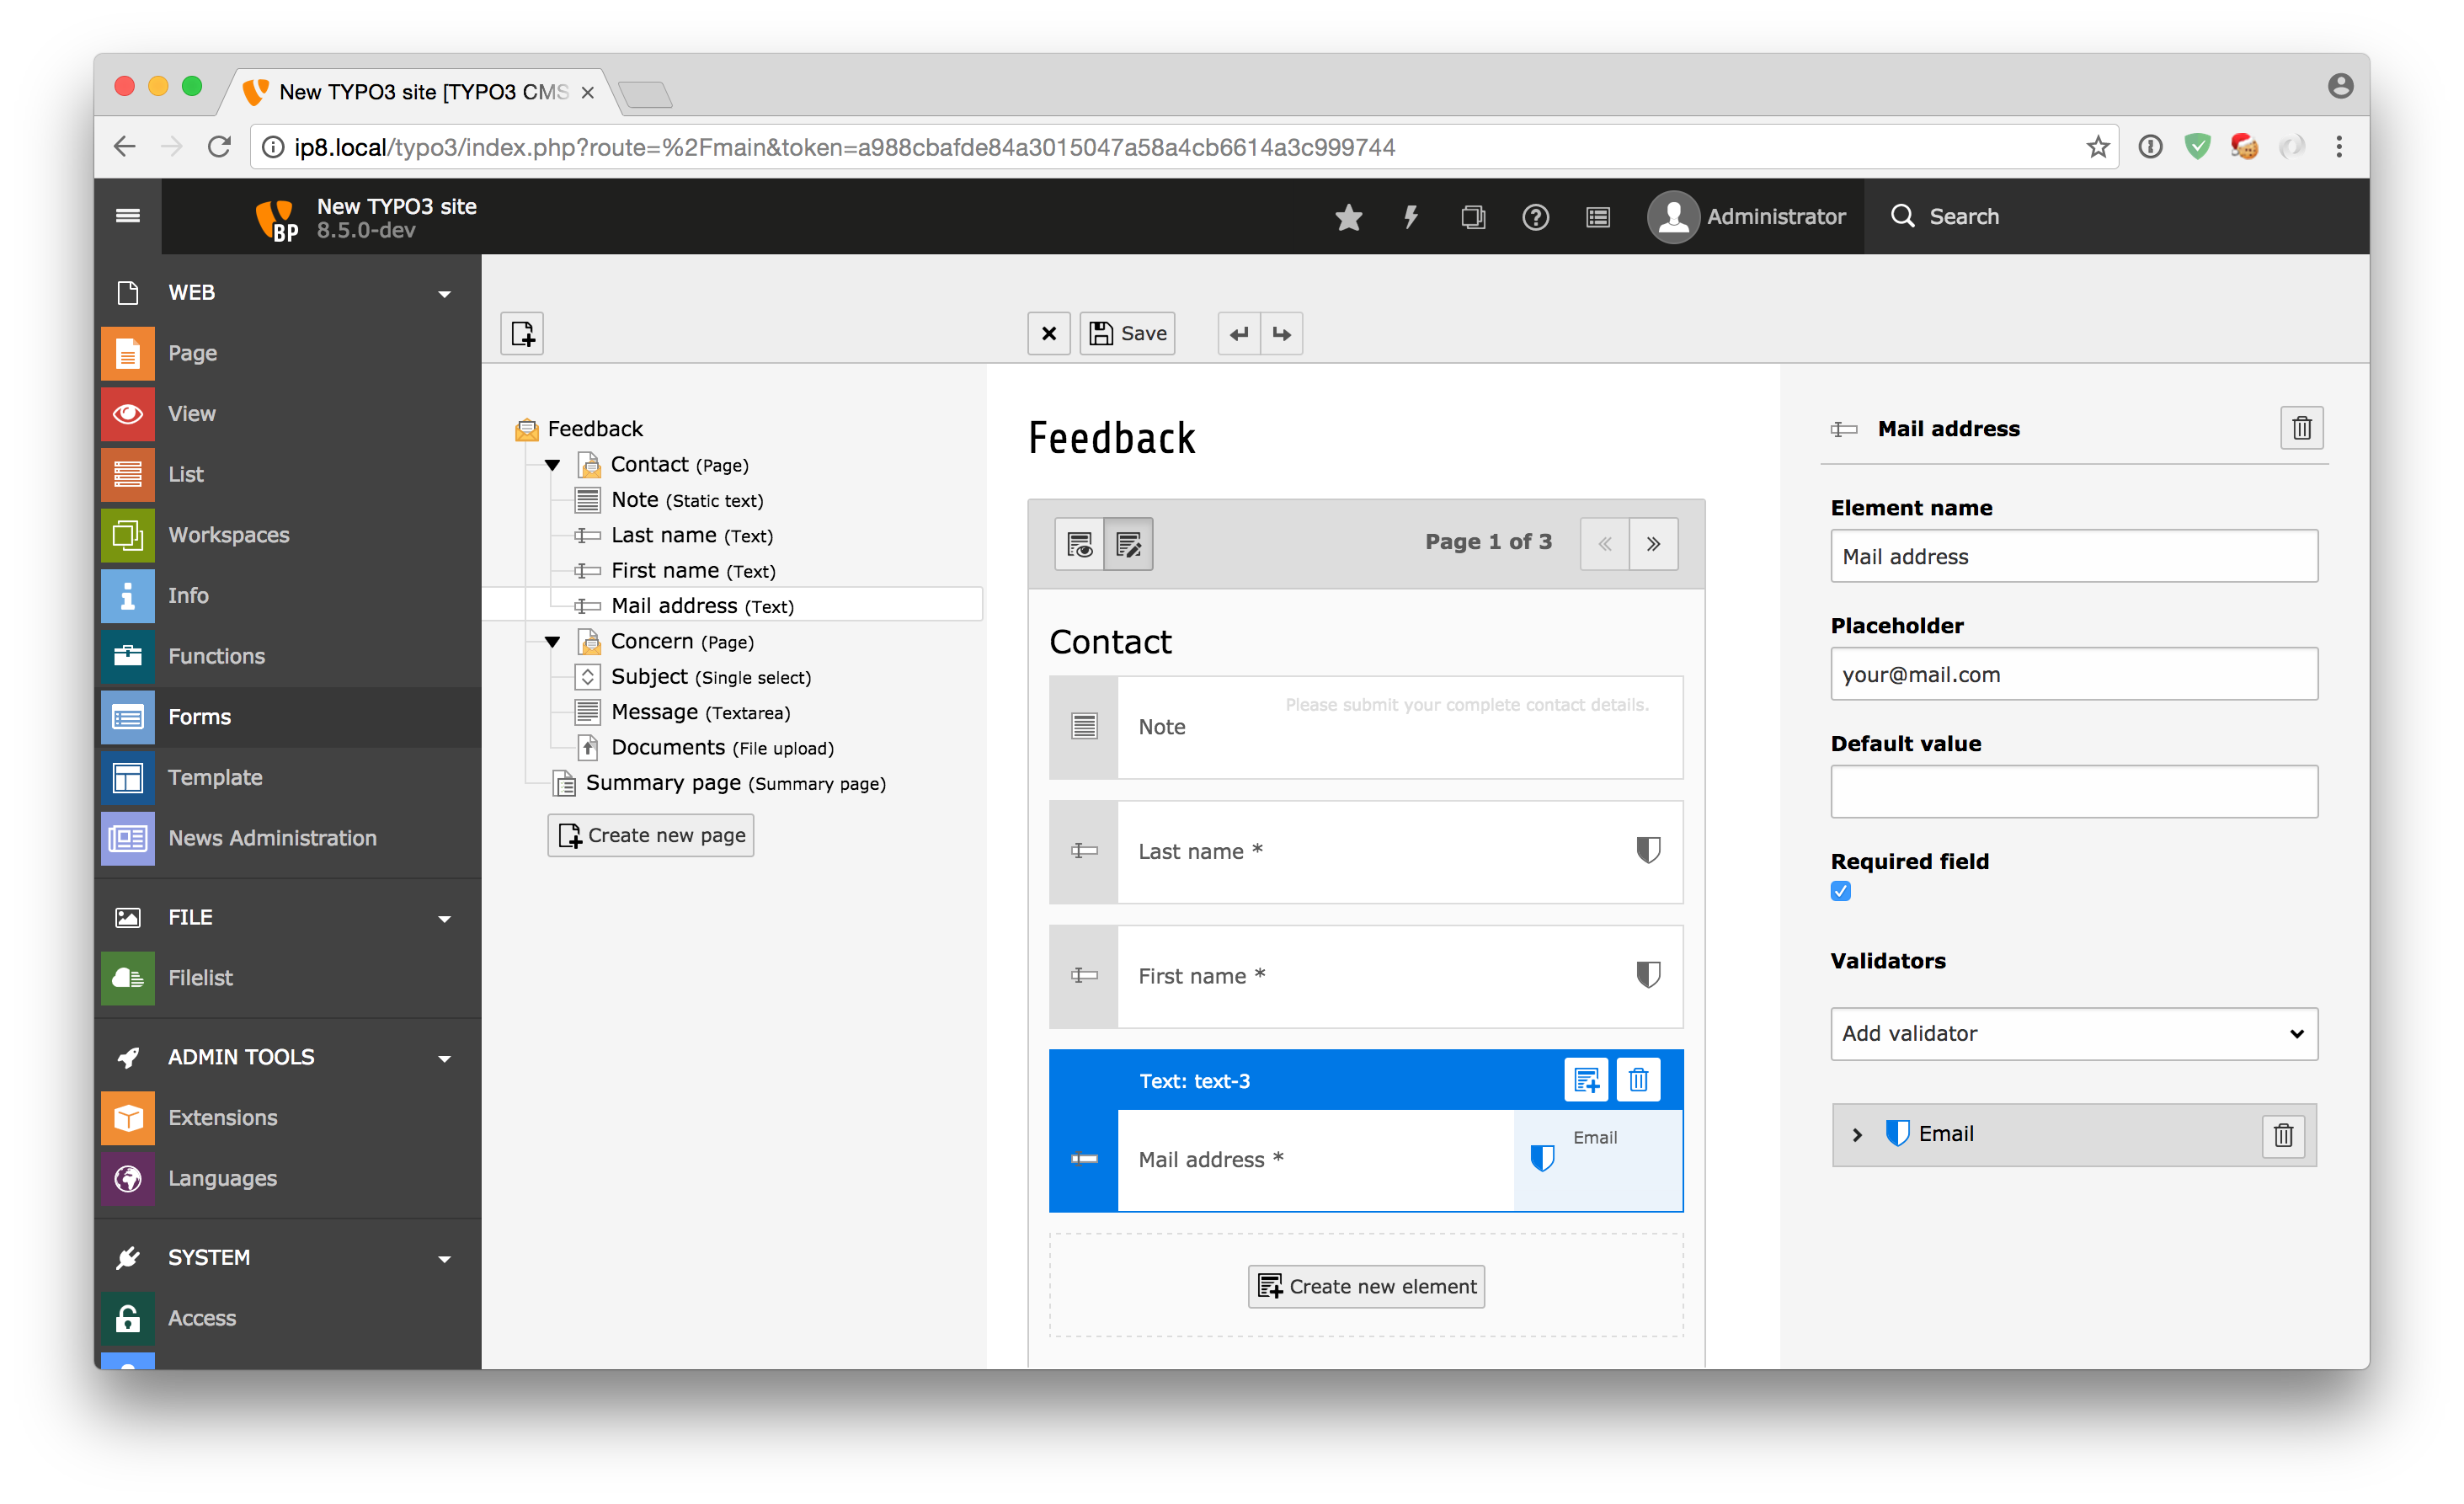
\includegraphics[width=0.8\linewidth]{FormFramework/form-framework-1.png}
	\end{figure}

\end{frame}

% ------------------------------------------------------------------------------
% LTXE-SLIDE-START
% LTXE-SLIDE-UID:		b91ec75b-7aa7b566-b523ca5f-f9ba3cde
% LTXE-SLIDE-TITLE:		#77910: New Form Framework (4)
% ------------------------------------------------------------------------------
\begin{frame}[fragile]
	\frametitle{Backend User Interface}
	\framesubtitle{Screenshot (2)}

	\begin{figure}
		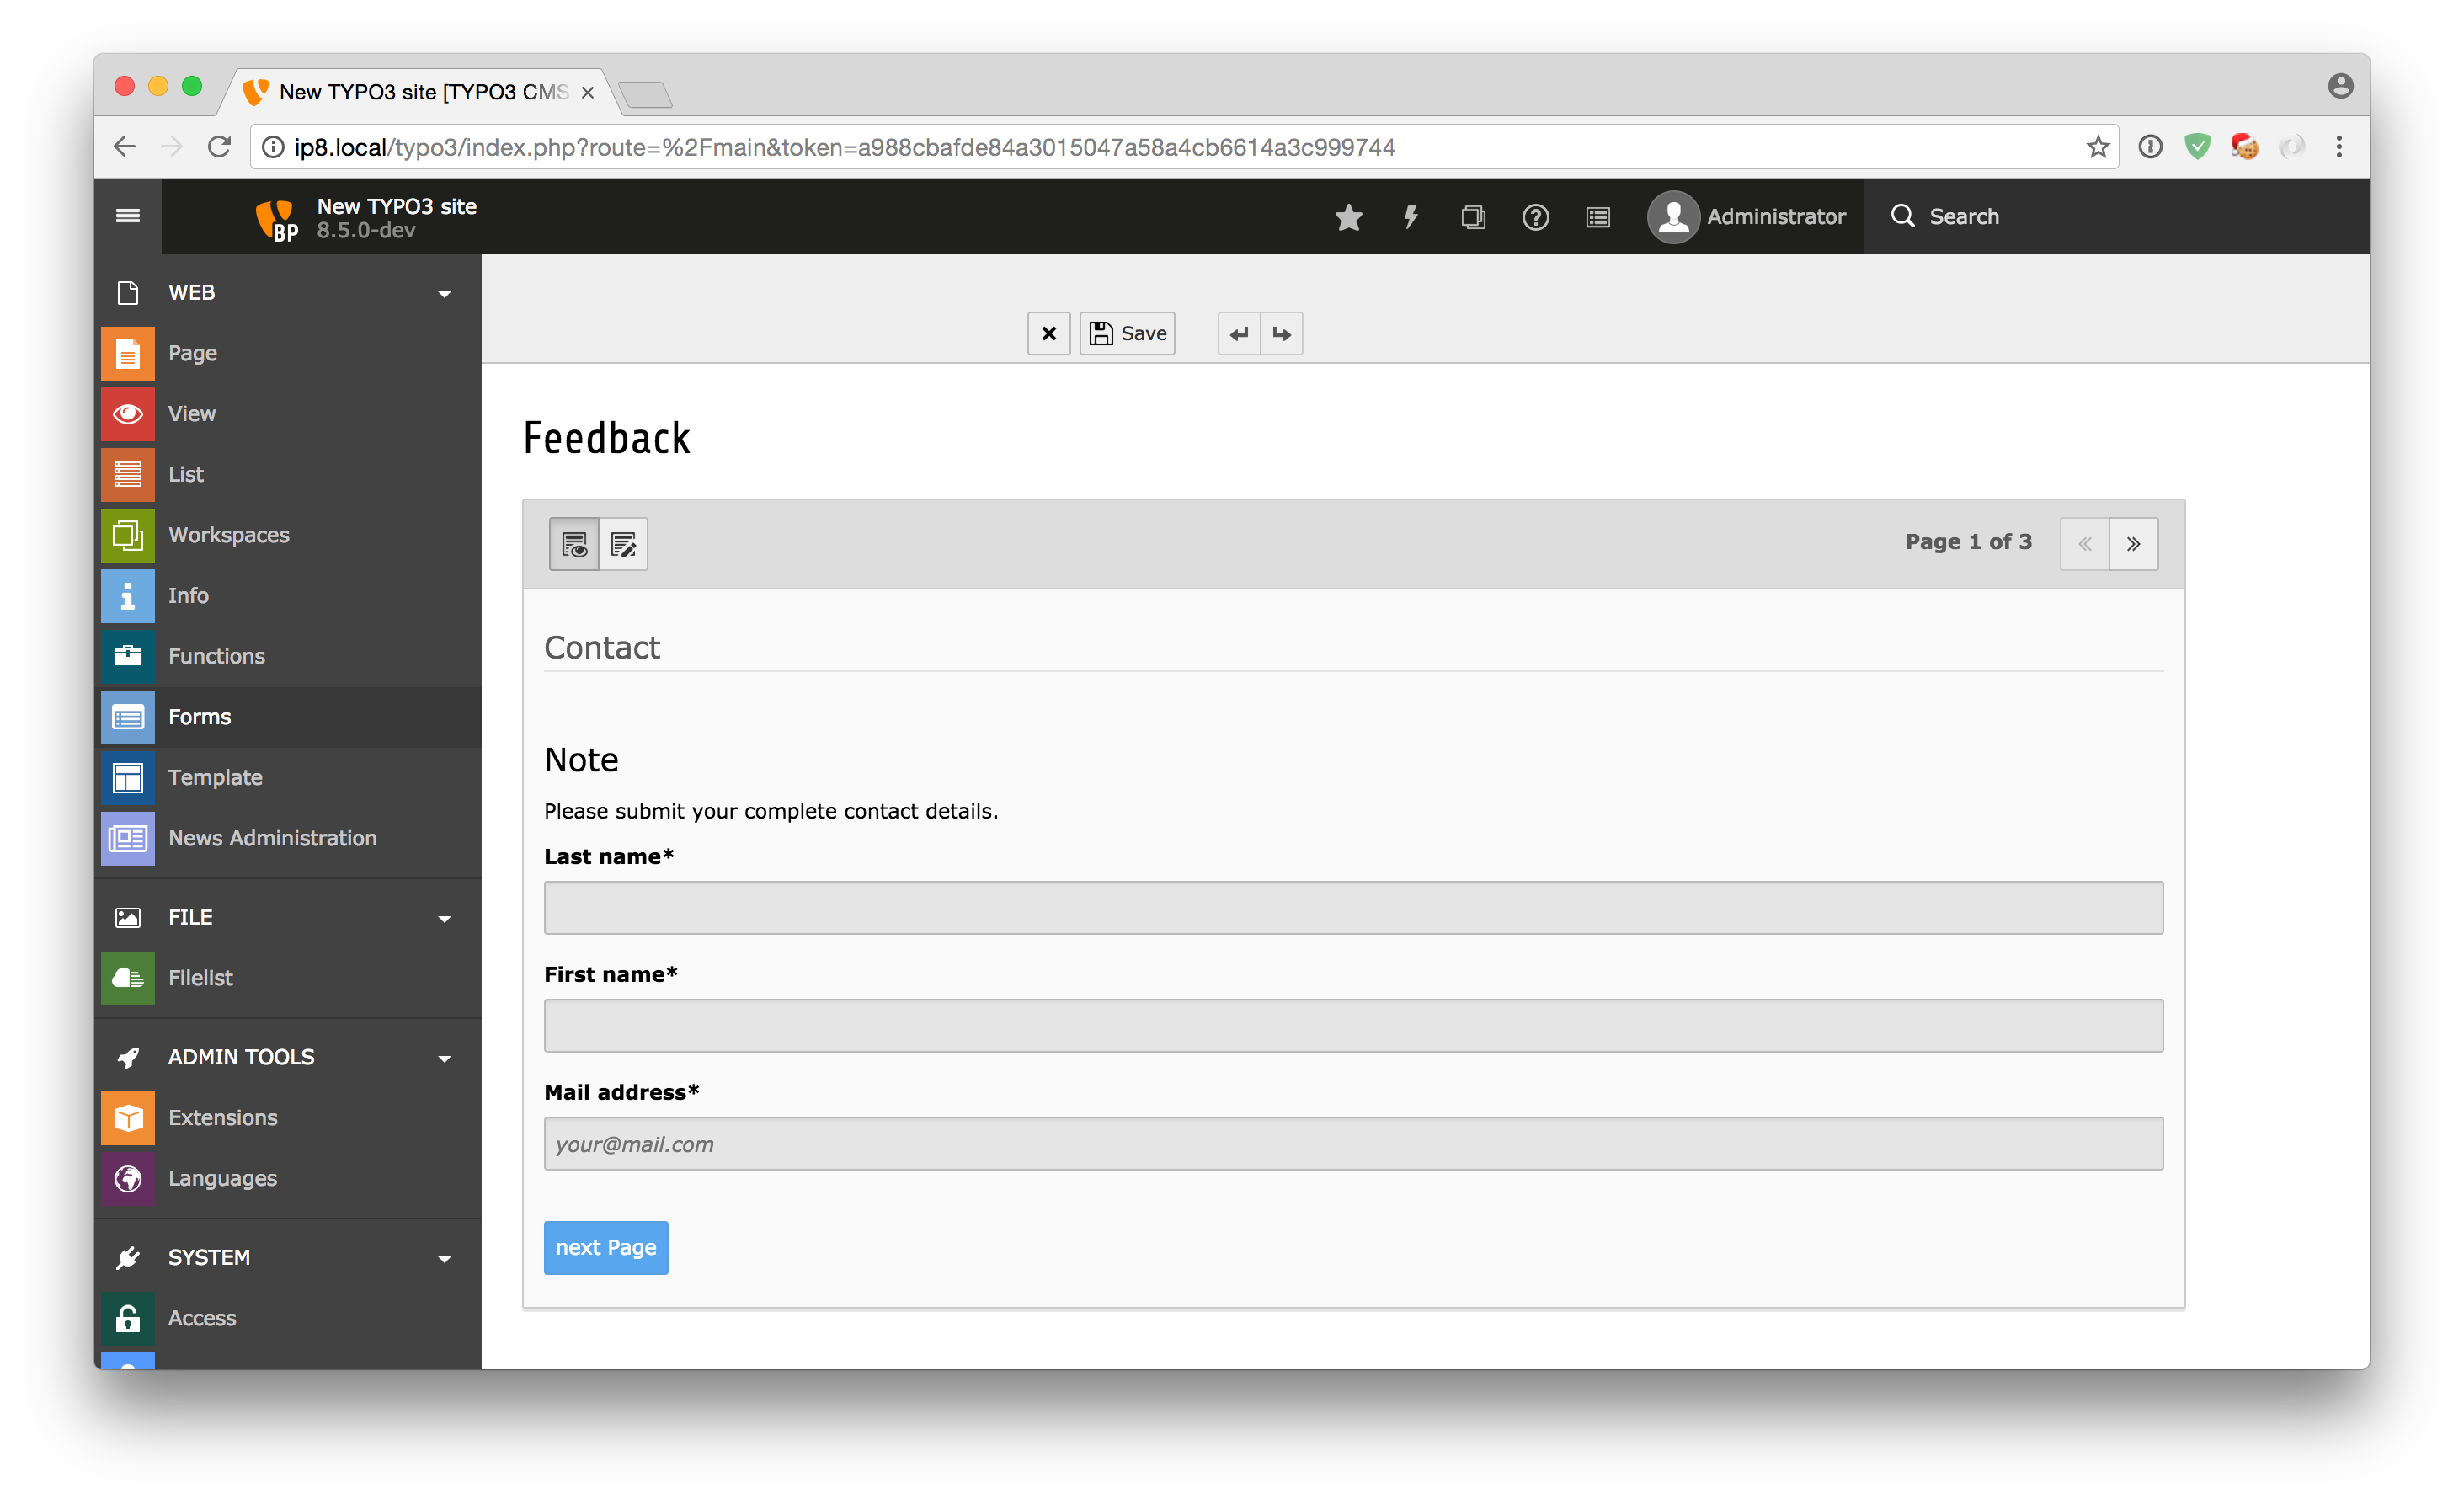
\includegraphics[width=0.8\linewidth]{FormFramework/form-framework-2.png}
	\end{figure}

\end{frame}

% ------------------------------------------------------------------------------
